
\mode<presentation> {

% The Beamer class comes with a number of default slide themes
% which change the colors and layouts of slides. Below this is a list
% of all the themes, uncomment each in turn to see what they look like.

%\usetheme{default}
%\usetheme{AnnArbor}
%\usetheme{Antibes}
%\usetheme{Bergen}
%\usetheme{Berkeley}
%\usetheme{Berlin}
%\usetheme{Boadilla}
%\usetheme{CambridgeUS}
%\usetheme{Copenhagen}
%\usetheme{Darmstadt}
%\usetheme{Dresden}
%\usetheme{Frankfurt}
%\usetheme{Goettingen}
%\usetheme{Hannover}
%\usetheme{Ilmenau}
%\usetheme{JuanLesPins}
%\usetheme{Luebeck}
%\usetheme{Madrid}
%\usetheme{Malmoe}
%\usetheme{Marburg}
%\usetheme{Montpellier}
\usetheme{PaloAlto}
%\usetheme{Pittsburgh}
%\usetheme{Rochester}
%\usetheme{Singapore}
%\usetheme{Szeged}
%\usetheme{Warsaw}

% As well as themes, the Beamer class has a number of color themes
% for any slide theme. Uncomment each of these in turn to see how it
% changes the colors of your current slide theme.

%\usecolortheme{albatross}
%\usecolortheme{beaver}
%\usecolortheme{beetle}
%\usecolortheme{crane}
%\usecolortheme{dolphin}
%\usecolortheme{dove}
%\usecolortheme{fly}
%\usecolortheme{lily}
%\usecolortheme{orchid}
%\usecolortheme{rose}
%\usecolortheme{seagull}
%\usecolortheme{seahorse}
%\usecolortheme{whale}
%\usecolortheme{wolverine}

%\setbeamertemplate{footline} % To remove the footer line in all slides uncomment this line
%\setbeamertemplate{footline}[page number] % To replace the footer line in all slides with a simple slide count uncomment this line

%\setbeamertemplate{navigation symbols}{} % To remove the navigation symbols from the bottom of all slides uncomment this line
}

% remove title and author from left panel
 \makeatletter
  \setbeamertemplate{sidebar \beamer@sidebarside}%{sidebar theme}
  {
    \beamer@tempdim=\beamer@sidebarwidth%
    \advance\beamer@tempdim by -6pt%
    \insertverticalnavigation{\beamer@sidebarwidth}%
    \vfill
    \ifx\beamer@sidebarside\beamer@lefttext%
    \else%
      \usebeamercolor{normal text}%
      \llap{\usebeamertemplate***{navigation symbols}\hskip0.1cm}%
      \vskip2pt%
    \fi%
  }%
\makeatother
% done remove title and author from left panel 

\hypersetup{colorlinks,citecolor=cyan}
\usepackage{graphicx} % Allows including images
\usepackage{booktabs} % Allows the use of \toprule, \midrule and \bottomrule in tables
\usepackage{natbib}
\usepackage{apalike}
\usepackage{comment}
% \usepackage{enumitem}
% \setlist[itemize]{topsep=0pt,before=\leavevmode\vspace{-1.5em}}
% \setlist[description]{style=nextline}
\usepackage{amsthm}
\usepackage{media9}
% \usepackage{multimedia}
\usepackage{hyperref}
\usepackage{tikz}
\tikzset{
     arrow/.style={-{Stealth[]}}
     }
\usetikzlibrary{positioning,arrows.meta}
\usetikzlibrary{shapes.geometric}

\setbeamertemplate{navigation symbols}{}%remove navigation symbols

\usepackage{setspace}

\newtheorem{probDef}{Definition}
\newtheorem*{probDef*}{Definition}
\newtheorem{claim}{Claim}
\newtheorem*{claim*}{Claim}
\newtheorem{probExample}{Example}
\newtheorem{probRule}{Rule}
\newtheorem{probAxiom}{Axiom}
\setbeamertemplate{theorems}[numbered]

\newtheorem{manualprobRuleinner}{Rule}
\newenvironment{manualProbRule}[1]{%
  \renewcommand\themanualprobRuleinner{#1}%
  \manualprobRuleinner
}{\endmanualprobRuleinner}

\newtheorem{manualprobExampleinner}{Example}
\newenvironment{manualProbExample}[1]{%
  \renewcommand\themanualprobExampleinner{#1}%
  \manualprobExampleinner
}{\endmanualprobExampleinner}

\newcounter{saveenumi}
\newcommand{\seti}{\setcounter{saveenumi}{\value{enumi}}}
\newcommand{\conti}{\setcounter{enumi}{\value{saveenumi}}}
\newcommand{\keepi}{\addtocounter{saveenumi}{-1}\setcounter{enumi}{\value{saveenumi}}}

%----------------------------------------------------------------------------------------
%	TITLE PAGE
%----------------------------------------------------------------------------------------

\title{Inference}

\author{Joaqu\'{i}n Rapela} % Your name
\institute[GCNU, UCL] % Your institution as it will appear on the bottom of every slide, may be shorthand to save space
{
Gatsby Computational Neuroscience Unit\\University College London % Your institution for the title page
}
\date{\today} % Date, can be changed to a custom date

\AtBeginSection[]
  {
     \begin{frame}<beamer>
     \frametitle{Contents}
         \tableofcontents[currentsection,hideallsubsections]
     \end{frame}
  }

\begin{document}

\begin{frame}
\titlepage % Print the title page as the first slide
\end{frame}

\begin{frame}
\frametitle{Contents} % Table of contents slide, comment this block out to remove it
\tableofcontents % Throughout your presentation, if you choose to use \section{} and \subsection{} commands, these will automatically be printed on this slide as an overview of your presentation
\end{frame}

\begin{frame}
\frametitle{Main reference} % Table of contents slide, comment this block out to remove it

    I will mainly follow chapters two \textit{Probability distributions} and
    three \textit{Linear models for regression} from
    \citet{bishop06}.

    \begin{center}
        \includegraphics[width=1.5in]{figures/bishop06Cover.png}
    \end{center}

\end{frame}

\begin{comment}
\begin{frame}
\frametitle{Main lecture goals}

    % \resizebox{5}{3}{%
    % \scalebox{0.7}{%
    \begin{figure}
        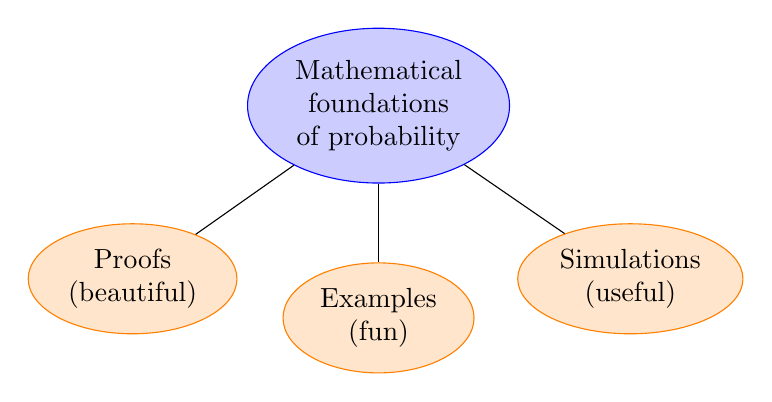
\begin{tikzpicture}
            % Place nodes
            \node[ellipse,align=center,anchor=north,fill=blue!20,draw=blue] (foundations) {Mathematical\\foundations\\of probability};
            \node[ellipse,align=center,anchor=north,fill=orange!20,draw=orange] [below left=of foundations] (proofs) {Proofs\\(beautiful)};
            \node[ellipse,align=center,anchor=north,fill=orange!20,draw=orange] [below=of foundations] (examples) {Examples\\(fun)};
            \node[ellipse,align=center,anchor=north,fill=orange!20,draw=orange] [below right=of foundations] (simulations) {Simulations\\(useful)};
            % Draw edges
            \path[-] (foundations) edge node [] {} (proofs);
            \path[-] (foundations) edge node [] {} (examples);
            \path[-] (foundations) edge node [] {} (simulations);
        \end{tikzpicture}
    \end{figure }

\end{frame}
\end{comment}

\section{The Gaussian distribution}

\begin{frame}
\frametitle{The Gaussian distribution}

    \begin{itemize}
        \item One-dimensional
        \begin{align*}
            \mathcal{N}(x|\mu,\sigma^2)=\frac{1}{(2\pi)^\frac{1}{2}(\sigma^2)^\frac{1}{2}}\exp\left\{-\frac{1}{2}\frac{(x-\mu)^2}{\sigma^2}\right\}
        \end{align*}
        \item D-dimensional
        \begin{align*}
            \mathcal{N}(\mathbf{x}|\boldsymbol{\mu},\Sigma)=\frac{1}{(2\pi)^{D/2}\Sigma^{\frac{1}{2}}}\exp\left\{-\frac{1}{2}(\mathbf{x}-\boldsymbol{\mu})^\intercal\Sigma^{-1}(\mathbf{x}-\boldsymbol{\mu})\right\}
        \end{align*}
    \end{itemize}

\end{frame}

\begin{frame}
    \frametitle{The Gaussian is the maximum entropy distribution
    \citep{coverAndThomas91}}

    \begin{probDef}[Differential entropy]
        The \textit{differential entropy} $h(X)$ of a continuous random
        variable X with a density $f(x)$ is defined as

        \begin{align*}
            h(X)=-\int_Sf(X)\log f(x)\ dx
        \end{align*}

        where $S$ is the support set of the random variable.
    \end{probDef}

    \begin{theorem}[The Gaussian is the maximum entropy distribution]
        Let the random vector $X\in\mathbb{R}^n$ have zero mean and covariance
        $K$. Then $h(X)\le\frac{1}{2}\log(2\pi e)^n|K|$, with equality if
        $X\sim\mathcal{N}(0,K)$.
    \end{theorem}

\end{frame}

\begin{frame}
    \frametitle{The central limit theorem \citep{papoulisAndPillai02}}

	\begin{theorem}[The central limit theorem]
		Given $n$ independent and identically distributed random vectors $\mathbf{X}_i$, with mean vector $\boldsymbol{\mu}=E\{\mathbf{X}_i\}$ and covariance matrix $\mathbf{\Sigma}$. Then

		\begin{align*}
			\sqrt{n}(\bar{\mathbf{X}}_n-\boldsymbol{\mu})\rightarrow\mathcal{N}(0,\Sigma)
		\end{align*}

		with convergence in distribution.
	\end{theorem}
\end{frame}

\begin{frame}
    \frametitle{Very useful properties of the Gaussian distribution \citep{bishop06}}

	\small
	\begin{theorem}[Marginals and conditionals of Gaussians are Gaussians]
		\label{thm:marginalOrConditionalOfGaussianIsGaussian}

		Given $\mathbf{x}=\left[\begin{array}{c}
									\mathbf{x}_a\\
									\mathbf{x}_b\\
								\end{array}\right]$ such that

		\begin{align*}
			p(\mathbf{x})&=\mathcal{N}\left(\mathbf{x}\left|
				\left[\begin{array}{c}
					      \boldsymbol{\mu}_a\\
						  \boldsymbol{\mu}_b\\
				   	  \end{array}\right],
				\left[\begin{array}{cc}
					      \Sigma_{aa} & \Sigma_{ab}\\
						  \Sigma_{ba} & \Sigma_{bb}\\
					  \end{array}\right]
			\right.\right)\\
			            &=\mathcal{N}\left(\mathbf{x}\left|
				\left[\begin{array}{c}
					      \boldsymbol{\mu}_a\\
						  \boldsymbol{\mu}_b\\
				   	  \end{array}\right],
				\left[\begin{array}{cc}
					      \Lambda_{aa} & \Lambda_{ab}\\
						  \Lambda_{ba} & \Lambda_{bb}\\
					  \end{array}\right]^{-1}
			\right.\right)
		\end{align*}
		Then
		\begin{align}
			p(\mathbf{x}_a|\mathbf{x}_b)&=\mathcal{N}\left(\mathbf{x}_a\left|\boldsymbol{\mu}_a-\Lambda_{aa}^{-1}\Lambda_{ab}(\mathbf{x}_b-\boldsymbol{\mu}_b),\Lambda_{aa}^{-1}\right.\right)\label{eq:gaussianCond1}\\
			                            &=\mathcal{N}\left(\mathbf{x}_a\left|\boldsymbol{\mu}_a+\Sigma_{ab}\Sigma_{bb}^{-1}(\mathbf{x}_b-\boldsymbol{\mu}_b),\Sigma_{aa}-\Sigma_{ab}\Sigma_{bb}^{-1}\Sigma_{ba}\right.\right)\label{eq:gaussianCond2}\\
            p(\mathbf{x}_b)&=\mathcal{N}\left(\mathbf{x}_b\left|\boldsymbol{\mu}_b,\Sigma_{bb}\right.\right)\label{eq:gaussianMarginal}
		\end{align}

	\end{theorem}
	\normalsize
\end{frame}

\begin{frame}
    \frametitle{Very useful properties of the Gaussian distribution \citep{bishop06}}

	\small
	\begin{theorem}[Marginals and conditionals of the linear Gaussian model]

		Given the linear Gaussian model

		\begin{align*}
			p(\mathbf{x})&=\mathcal{N}(\mathbf{x}|\boldsymbol{\mu},\Lambda^{-1})\\
			p(\mathbf{y}|\mathbf{x})&=\mathcal{N}(\mathbf{y}|A\boldsymbol{\mu}+\mathbf{b},L^{-1})
		\end{align*}

		Then

		\begin{align*}
			p(\mathbf{y})&=\mathcal{N}(\mathbf{y}|A\boldsymbol{\mu}+\mathbf{b},L^{-1}+A\Lambda^{-1}\Sigma^\intercal)\\
			p(\mathbf{x}|\mathbf{y})&=\mathcal{N}(\mathbf{x}|\Sigma\{A^\intercal L(\mathbf{y}-\mathbf{b})+\Sigma\boldsymbol{\mu}\},\Sigma)
		\end{align*}

		where

		\begin{align*}
			\Sigma=(\Lambda+A^\intercal LA)^{-1}
		\end{align*}

	\end{theorem}
	\normalsize
\end{frame}

\begin{frame}
    \frametitle{Very useful properties of the Gaussian distribution \citep{bishop06}}

	The conditional, $p(\mathbf{x}|\mathbf{y})$, of the linear Gaussian model is the fundamental result used in the derivation of

	\begin{enumerate}

		\item Bayesian linear regression~\citep{bishop06},

		\item Gaussian process regression~\citep{williamsAndRasmussen06},

		\item Gaussian process factor analysis~\citep{yuEtAl09},

		\item linear dynamical systems~\citep{durbinAndKoopman12}.

	\end{enumerate}

\end{frame}

\begin{frame}
    \frametitle{Proof: the conditional of a Gaussian is a Gaussian (Theorem~\ref{thm:marginalOrConditionalOfGaussianIsGaussian}, Eq.~\ref{eq:gaussianCond1})}

	\begin{claim}[Quadratic form of Gaussian log pdf]
		\label{claim:quadratricFormOfGaussianPDF}

		$p(\mathbf{x})$ is a Gaussian pdf with mean $\boldsymbol{\mu}$ and precision matrix $\Lambda$ if and only if $\int p(\mathbf{x}) d\mathbf{x}=1$ and

		\begin{align}
			\log p(\mathbf{x})=-\frac{1}{2}(\mathbf{x}^\intercal\Lambda\mathbf{x}-2\mathbf{x}^\intercal\Lambda\boldsymbol{\mu})+K\label{eq:gaussianQuadratic}
		\end{align}

		where $K$ is a constant that does not depend on $\mathbf{x}$.

	\end{claim}

\end{frame}

\begin{frame}
    \frametitle{Proof: the conditional of a Gaussian is a Gaussian (Theorem~\ref{thm:marginalOrConditionalOfGaussianIsGaussian}, Eq.~\ref{eq:gaussianCond1})}

	\begin{proof}[Proof of Claim~\ref{claim:quadratricFormOfGaussianPDF}]

		\scriptsize
		\begin{description}
			\item[$\rightarrow)$]

				\begin{align*}
					p(\mathbf{x})&=\frac{1}{(2\pi)^{D/2}\Lambda^{-\frac{1}{2}}}\exp\left\{-\frac{1}{2}(\mathbf{x}-\boldsymbol{\mu})^\intercal\Lambda(\mathbf{x}-\boldsymbol{\mu})\right\}\\
					\log p(\mathbf{x})&=-\frac{1}{2}(\mathbf{x}-\boldsymbol{\mu})^\intercal\Lambda(\mathbf{x}-\boldsymbol{\mu})-\log ((2\pi)^{D/2}\Lambda^{-\frac{1}{2}})\\
					                  &=-\frac{1}{2}(\mathbf{x}^\intercal\Lambda\mathbf{x}-2\mathbf{x}^\intercal\Lambda\boldsymbol{\mu})-\frac{1}{2}\boldsymbol{\mu}^\intercal\Lambda\boldsymbol{\mu}-\log ((2\pi)^{D/2}\Lambda^{-\frac{1}{2}})\\
					                  &=-\frac{1}{2}(\mathbf{x}^\intercal\Lambda\mathbf{x}-2\mathbf{x}^\intercal\Lambda\boldsymbol{\mu})+K
				\end{align*}
				with $K=-\frac{1}{2}\boldsymbol{\mu}^\intercal\Lambda\boldsymbol{\mu}-\log ((2\pi)^{D/2}\Lambda^{-\frac{1}{2}})$.
				\phantom\qedhere
		\end{description}
		\normalsize
	\end{proof}
\end{frame}

\begin{frame}
    \frametitle{Proof: the conditional of a Gaussian is a Gaussian (Theorem~\ref{thm:marginalOrConditionalOfGaussianIsGaussian}, Eq.~\ref{eq:gaussianCond1})}

	\begin{proof}[Proof of Claim~\ref{claim:quadratricFormOfGaussianPDF}]

		\scriptsize
		\begin{description}
			\item[$\leftarrow)$]

				\begin{align}
					\log p(\mathbf{x})=&-\frac{1}{2}(\mathbf{x}^\intercal\Lambda\mathbf{x}-2\mathbf{x}^\intercal\Lambda\boldsymbol{\mu})+K\nonumber\\
					\log p(\mathbf{x})=&-\frac{1}{2}(\mathbf{x}^\intercal\Lambda\mathbf{x}-2\mathbf{x}^\intercal\Lambda\boldsymbol{\mu})-\frac{1}{2}\boldsymbol{\mu}^\intercal\Lambda\boldsymbol{\mu}-\log ((2\pi)^{D/2}\Lambda^{-\frac{1}{2}})\nonumber\\
					                   &+K+\frac{1}{2}\boldsymbol{\mu}^\intercal\Lambda\boldsymbol{\mu}+\log ((2\pi)^{D/2}\Lambda^{-\frac{1}{2}})\nonumber\\
					                  =&-\frac{1}{2}(\mathbf{x}-\boldsymbol{\mu})^\intercal\Lambda(\mathbf{x}-\boldsymbol{\mu})-\log ((2\pi)^{D/2}\Lambda^{-\frac{1}{2}})\nonumber\\
					                   &+K+\frac{1}{2}\boldsymbol{\mu}^\intercal\Lambda\boldsymbol{\mu}+\log ((2\pi)^{D/2}\Lambda^{-\frac{1}{2}})\nonumber\\
					                  =&\log N(\mathbf{x}|\boldsymbol{\mu},\Lambda)+K+\frac{1}{2}\boldsymbol{\mu}^\intercal\Lambda\boldsymbol{\mu}+\log ((2\pi)^{D/2}\Lambda^{-\frac{1}{2}})\nonumber\\
					     p(\mathbf{x})=&N(\mathbf{x}|\boldsymbol{\mu},\Lambda)\exp\left(K+\frac{1}{2}\boldsymbol{\mu}^\intercal\Lambda\boldsymbol{\mu}+\log ((2\pi)^{D/2}\Lambda^{-\frac{1}{2}})\right)\label{eq:quadratricFormOfGaussianPDF_almostFinal}
				\end{align}
				\phantom\qedhere
		\end{description}
		\normalsize
	\end{proof}
\end{frame}

\begin{frame}
    \frametitle{Proof: the conditional of a Gaussian is a Gaussian (Theorem~\ref{thm:marginalOrConditionalOfGaussianIsGaussian}, Eq.~\ref{eq:gaussianCond1})}

	\begin{proof}[Proof of Claim~\ref{claim:quadratricFormOfGaussianPDF}]

		\scriptsize
		\begin{description}
			\item[$\leftarrow)$ cont]
				\begin{align*}
					1&=\int p(\mathbf{x})d\mathbf{x}\\
					 &=\int N(\mathbf{x}|\boldsymbol{\mu},\Lambda)\exp\left(K+\frac{1}{2}\boldsymbol{\mu}^\intercal\Lambda\boldsymbol{\mu}+\log ((2\pi)^{D/2}\Lambda^{-\frac{1}{2}})\right)d\mathbf{x}\\
					 &=\exp\left(K+\frac{1}{2}\boldsymbol{\mu}^\intercal\Lambda\boldsymbol{\mu}+\log ((2\pi)^{D/2}\Lambda^{-\frac{1}{2}})\right)\int N(\mathbf{x}|\boldsymbol{\mu},\Lambda)d\mathbf{x}\\
					 &=\exp\left(K+\frac{1}{2}\boldsymbol{\mu}^\intercal\Lambda\boldsymbol{\mu}+\log ((2\pi)^{D/2}\Lambda^{-\frac{1}{2}})\right)
				\end{align*}
				From Eq.~\ref{eq:quadratricFormOfGaussianPDF_almostFinal} then $p(\mathbf{x})=N(\mathbf{x}|\boldsymbol{\mu},\Lambda)$.
		\end{description}
		\normalsize
	\end{proof}
\end{frame}

\begin{frame}
    \frametitle{Proof: the conditional of a Gaussian is a Gaussian (Theorem~\ref{thm:marginalOrConditionalOfGaussianIsGaussian}, Eq.~\ref{eq:gaussianCond1})}

	\begin{proof}[Proof of Theorem~\ref{thm:marginalOrConditionalOfGaussianIsGaussian}, Eq.~\ref{eq:gaussianCond1}]

		\scriptsize
		\begin{align*}
			p(\mathbf{x}_a|\mathbf{x}_b)&=\frac{p(\mathbf{x}_a,\mathbf{x}_b)}{p(\mathbf{x}_b)}=\frac{p(\mathbf{x})}{p(\mathbf{x}_b)}\\
			\log p(\mathbf{x}_a|\mathbf{x}_b)&=\log p(\mathbf{x})-\log p(\mathbf{x}_b)=\log p(\mathbf{x})+K
		\end{align*}

		Therefore, the terms of $\log p(\mathbf{x}_a|\mathbf{x}_b)$ that depend on $\mathbf{x}_a$ are those of $\log p(\mathbf{x})$.

		Steps for the proof:

		\begin{enumerate}
			\item isolate the terms of $\log p(\mathbf{x})$ that depend on $\mathbf{x}_a$,
			\item notice that these term has the quadratic form of Claim~\ref{claim:quadratricFormOfGaussianPDF}, therefore $p(\mathbf{x}_a|\mathbf{x}_b)$ is Gaussian,
			\item identify $\boldsymbol{\mu}$ and $\Lambda$ in this quadratic form.
		\end{enumerate}

		\phantom\qedhere
		\normalsize
	\end{proof}
\end{frame}

\begin{frame}
    \frametitle{Proof: the conditional of a Gaussian is a Gaussian (Theorem~\ref{thm:marginalOrConditionalOfGaussianIsGaussian}, Eq.~\ref{eq:gaussianCond1})}

	\begin{proof}[Proof of Theorem~\ref{thm:marginalOrConditionalOfGaussianIsGaussian}, Eq.~\ref{eq:gaussianCond1}]

		\scriptsize
		\begin{align*}
			p(\mathbf{x})&=\frac{1}{(2\pi)^{D/2}|\Lambda|^{1/2}}\exp\left(-\frac{1}{2}(\mathbf{x}-\boldsymbol{\mu})^\intercal\Lambda(\mathbf{x}-\boldsymbol{\mu})\right)\\
			\log p(\mathbf{x})=&-\frac{1}{2}(\mathbf{x}-\boldsymbol{\mu})^\intercal\Lambda(\mathbf{x}-\boldsymbol{\mu})+K_1\\
			                  =&-\frac{1}{2}[(\mathbf{x}_a-\boldsymbol{\mu}_a)^\intercal,(\mathbf{x}_b-\boldsymbol{\mu}_b)^\intercal]\left[\begin{array}{cc}
							                                                                                                                   \Lambda_{aa} & \Lambda_{ab}\\
							                                                                                                                   \Lambda_{ba} & \Lambda_{bb}
																																	       \end{array}\right]
																																	 \left[\begin{array}{c}
																																	           \mathbf{x}_a-\boldsymbol{\mu}_a\\
																																	           \mathbf{x}_b-\boldsymbol{\mu}_b\\
																																			\end{array}\right]
																																	 +K_1\\
			                  =&-\frac{1}{2}\left\{(\mathbf{x}_a-\boldsymbol{\mu}_a)^\intercal\Lambda_{aa}(\mathbf{x}_a-\boldsymbol{\mu}_a)+2(\mathbf{x}_a-\boldsymbol{\mu}_a)^\intercal\Lambda_{ab}(\mathbf{x}_b-\boldsymbol{\mu}_b)\right.\\
							   &\left.+(\mathbf{x}_b-\boldsymbol{\mu}_b)^\intercal\Lambda_{bb}(\mathbf{x}_b-\boldsymbol{\mu}_b)\right\}+K_1\\
			                  =&-\frac{1}{2}\left\{\mathbf{x}_a^\intercal\Lambda_{aa}\mathbf{x}_a-2\mathbf{x}_a^\intercal(\Lambda_{aa}\boldsymbol{\mu}_a-\Lambda_{ab}(\mathbf{x}_b-\boldsymbol{\mu}_b))\right\}+K_2\\
			                  =&-\frac{1}{2}\left\{\mathbf{x}_a^\intercal\Lambda_{aa}\mathbf{x}_a-2\mathbf{x}_a^\intercal\Lambda_{aa}(\boldsymbol{\mu}_a-\Lambda_{aa}^{-1}\Lambda_{ab}(\mathbf{x}_b-\boldsymbol{\mu}_b))\right\}+K_2
		\end{align*}
		Comparing the last equation with Eq.~\ref{eq:gaussianQuadratic} we see that $\Lambda=\Lambda_{aa}$, $\boldsymbol{\mu}=\boldsymbol{\mu}_a-\Lambda_{aa}^{-1}\Lambda_{ab}(\mathbf{x}_b-\boldsymbol{\mu}_b)$ and conclude that $p(\mathbf{x}_a|\mathbf{x}_b)=\mathcal{N}(\mathbf{x}_a|\boldsymbol{\mu}_a-\Lambda_{aa}^{-1}\Lambda_{ab}(\mathbf{x}_b-\boldsymbol{\mu}_b),\Lambda_{aa})$
		\normalsize
	\end{proof}
\end{frame}

\begin{frame}
    \frametitle{Proof: the conditional of a Gaussian is a Gaussian (Theorem~\ref{thm:marginalOrConditionalOfGaussianIsGaussian}, Eq.~\ref{eq:gaussianCond2})}

	\begin{claim}[Inverse of a partitioned matrix]
		\begin{align}
			\left(\begin{array}{cc}
				      A & B\\
				      C & D
				  \end{array}^{-1}\right)=
			\left(\begin{array}{cc}
				      M         & -MBD^{-1}\\
					  -D^{-1}CM & D^{-1} + D^{-1}CMBD^{-1}
				  \end{array}\right)\label{eq:inversePartitionedMatrix}
		\end{align}
		where
		\begin{align*}
			M = (A - BD^{-1}C)^{-1}
		\end{align*}
	\end{claim}
	\begin{proof}
		\scriptsize
		Exercise. Hint: verify that the multiplication of the inverse of the matrix in the right hand side of Eq.~\ref{eq:inversePartitionedMatrix} with the matrix in the left hand side of the same equation is the identiy matrix.
		\phantom\qedhere
		\normalsize
	\end{proof}
\end{frame}

\begin{frame}
    \frametitle{Proof: the conditional of a Gaussian is a Gaussian (Theorem~\ref{thm:marginalOrConditionalOfGaussianIsGaussian}, Eq.~\ref{eq:gaussianCond2})}

	\begin{proof}[Proof of Theorem~\ref{thm:marginalOrConditionalOfGaussianIsGaussian}, Eq.~\ref{eq:gaussianCond2}]
		\scriptsize
		Using the definition
		\begin{align*}
			\left(\begin{array}{cc}
				      \Sigma_{aa} & \Sigma_{ab}\\
				      \Sigma_{ba} & \Sigma_{bb}
                  \end{array}\right)^{-1}=
			\left(\begin{array}{cc}
				      \Lambda_{aa} & \Lambda_{ab}\\
				      \Lambda_{ba} & \Lambda_{bb}
                  \end{array}\right)
		\end{align*}
		and using Eq.~\ref{eq:inversePartitionedMatrix}, we obtain
		\begin{align*}
			\Lambda_{aa}&=(\Sigma_{aa}-\Sigma_{ab}\Sigma_{bb}^{-1}\Sigma_{ba})^{-1}\\
			\Lambda_{ab}&=-(\Sigma_{aa}-\Sigma_{ab}\Sigma_{bb}^{-1}\Sigma_{ba})^{-1}\Sigma_{ab}\Sigma_{bb}^{-1}
		\end{align*}
		Replacing the above equations in Eq.~\ref{eq:gaussianCond1} we obtain Eq.~\ref{eq:gaussianCond2}.
		\normalsize
	\end{proof}

\end{frame}

\section{Linear models for regression}

\begin{frame}
    \frametitle{Linear regression example}

	\begin{center}
		\includegraphics[width=2.2in]{figures/visVesIntegration.png}
	\end{center}
	\hfill\href{https://www.biorxiv.org/content/10.1101/2021.01.22.427789v4.abstract}{Keshavarzi et al., 2021}
	\begin{columns}
		\onslide<2->{
		\begin{column}{0.5\textwidth}
			\begin{center}
				\includegraphics[width=1.5in]{figures/spikeRateVsabsSpeedV1VisVes.png}
			\end{center}
		\end{column}
		}
		\onslide<3->{
		\begin{column}{0.5\textwidth}
			\textcolor{blue}{Is there a linear relation between the speed of rotation and the firing rate of visual cells?}
		\end{column}
		}
	\end{columns}
\end{frame}

\begin{frame}
    \frametitle{Linear regression model}

	\scriptsize
	\begin{description}
		\item[simple linear regression model]
			\begin{align*}
                y(x_i, \mathbf{w})&=w_0+w_1x_i
				                   =\raisebox{0.60em}{$[1,x_i]$}
									\left[\begin{array}{c}
								        w_0\\
								        w_1
								    \end{array}\right]
				                   =\raisebox{0.60em}{$[\phi_0(x_i),\phi_1(x_i)]$}
									\left[\begin{array}{c}
								        w_0\\
								        w_1
								    \end{array}\right]\\
                                  & =
									\boldsymbol{\phi}(x_i)^\intercal\mathbf{w}
			\end{align*}
		\item[polynomial regression model]
			\begin{align*}
				y(x_i, \mathbf{w})&=w_0+w_1x_i+w_2x_i^2+w_3x_i^3
				                   =\raisebox{1.80em}{$[1,x_i,x_i^2,x_i^3]$}
									\left[\begin{array}{c}
								        w_0\\
								        w_1\\
								        w_2\\
								        w_3
								    \end{array}\right]\\
				                  &=\raisebox{1.80em}{$[\phi_0(x_i),\phi_1(x_i),\phi_2(x_i),\phi_3(x_i)]$}
									\left[\begin{array}{c}
								        w_0\\
								        w_1\\
								        w_2\\
								        w_3
								    \end{array}\right]=
									\boldsymbol{\phi}(x_i)^\intercal\mathbf{w}
			\end{align*}
		\item[basis functions regression model]
			\begin{align*}
				y(x_i,
                \mathbf{w})&=\boldsymbol{\phi}(x_i)^\intercal\mathbf{w}=\sum_{j=1}^Mw_j\phi_j(x_i)
			\end{align*}
	\end{description}
	\normalsize
\end{frame}

\begin{frame}
    \frametitle{Linear regression model}

    \scriptsize
    \begin{align*}
        \mathbf{y}(\mathbf{x},\mathbf{w})&=
            \left[\begin{array}{c}
                      y(x_1,\mathbf{w})\\
                      y(x_2,\mathbf{w})\\
                      \ldots\\
                      y(x_N,\mathbf{w})
                  \end{array}\right]=
            \left[\begin{array}{cccc}
                      \phi_1(x_1)&\phi_2(x_1)&\ldots&\phi_M(x_1)\\
                      \phi_1(x_2)&\phi_2(x_2)&\ldots&\phi_M(x_2)\\
                      \vdots     &\vdots     &\ldots&\vdots\\
                      \phi_1(x_N)&\phi_2(x_N)&\ldots&\phi_M(x_N)
            \end{array}\right]\left[\begin{array}{c}
                                        w_1\\
                                        w_2\\
                                        \vdots\\
                                        w_M
                                    \end{array}\right]\\
                                         &=\boldsymbol{\Phi}\mathbf{w}
    \end{align*}

    where
    $\mathbf{y}(\mathbf{x},\mathbf{w})\in\mathbb{R}^N,\boldsymbol{\Phi}\in\mathbb{R}^{N\times M},\mathbf{w}\in\mathbb{R}^M$.
    \normalsize
\end{frame}

\begin{frame}
    \frametitle{Basis functions for regression}

		\begin{center}
			\includegraphics[width=3.5in]{figures/basisFunctions.png}
		\end{center}
        \hfill\citet{bishop06}

        \begin{description}
            \item[polynomial] $\phi_i(x)=x^i$
            \item[Gaussian] $\phi_i(x)=\exp(-\frac{(x-\mu_i)^2}{2\sigma^2})$
            \item[sigmoidal]
                $\phi_i(x)=\frac{1}{1+\exp(-\frac{x-\mu_i}{\sigma^2})}$
        \end{description}
\end{frame}

\begin{frame}
    \frametitle{Least-squares estimation of model parameters
    \citep{trefethenAndBau97}}

    \scriptsize
    \begin{probDef}[Least-squares problem]
        Given $\boldsymbol{\Phi}\in\mathbb{R}^{N\times M},N\ge
        M,\mathbf{y}\in\mathbb{R}^N$, find $\mathbf{w}\in\mathbb{R}^M$ such that $||\mathbf{y}-\boldsymbol{\Phi}\boldsymbol{w}||_2$ is minimized.
    \end{probDef}
    \begin{theorem}[Least-squares solution]
        Let $\boldsymbol{\Phi}\in\mathbb{R}^{N\times M} (N\ge M)$ and
        $\mathbf{y}\in\mathbb{R}^N$ be given. A vector
        $\mathbf{w}\in\mathbb{R}^M$ minimizes
        $||\mathbf{r}||_2=||\mathbf{y}-\boldsymbol{\Phi}\mathbf{w}||_2$, thereby solving the
        least-squares problem, if and only if
        $\mathbf{r}\perp\text{range}(\boldsymbol{\Phi})$, that is,
        $\boldsymbol{\Phi}^\intercal\mathbf{r}=0$,
        or equivalently,
        $\boldsymbol{\Phi}^\intercal\boldsymbol{\Phi}\mathbf{w}=\boldsymbol\Phi^\intercal\mathbf{y}$,
        or again equivalently,
        $P\mathbf{y}=\boldsymbol{\Phi}\mathbf{w}$.
    \end{theorem}
	\begin{center}
		\includegraphics[width=2.5in]{figures/leastSquares.png}
	\end{center}

    \normalsize

    \note{
    Given a set of $N$ observations, $\mathbf{y}$, $N>M$, we want to find model
    parameters $\mathbf{w}$ such that the model outputs,
    $\mathbf{y}(\mathbf{x},\mathbf{w})$ equal the observations. This is
    generally impossible, because the degrees of freedom of the boservations,
    $N$, is generally larger than the degrees of freedom of the model
    $\mathbf{y}(\mathbf{x},\mathbf{w})$, $M$. We instead solve the following
    least-squares probem.
    }
\end{frame}

\begin{frame}
    \frametitle{References}

    \tiny{
        \bibliographystyle{apalike}
        \bibliography{probability,informationTheory,machineLearning,gaussianProcesses,latentsVariablesModels,linearDynamicalSystems,numericalMethods}
    }
\end{frame}

\begin{comment}
\end{comment}

\end{document}

